%%% ====================================================================
%%% Início da parte textual do documento.


%%% Configuração do espaçamento entre títulos e texto
\setlength{\afterchapskip}{1.5cm minus \baselineskip}


\chapter{Resultados}
\label{cha:resultados}

Esse capítulo contém os resultados da aplicação e dos estudos de casos aplicados.

\section{Aplicação}

\subsection{Diagrama de Classes}

Com auxílio da ferramenta \textit{Astah Community}, foi desenvolvido o seguinte Diagrama de Classes, apresentado na figura \ref{fig:diagramaClasses}:

\begin{figure}[H]
	\centering
	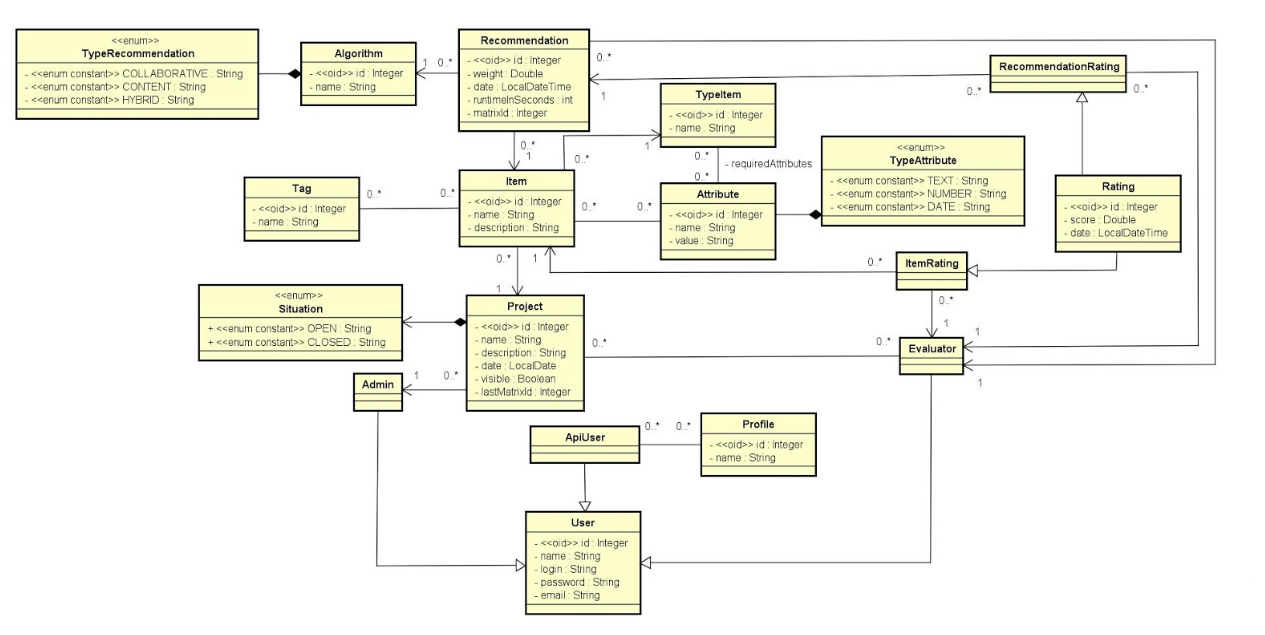
\includegraphics[width=1\linewidth]{imagens/diagramaClasses.PNG}
	\caption[Diagrama de Classes]{Diagrama de Classes}
    \label{fig:diagramaClasses}
\end{figure}

\subsection{API de Recomendação}

Foi desenvolvido uma aplicação backend aberta para uso e modificações. O código fonte de aplicação está disponível no \href{https://github.com/herikLorencao/srh-backend}{GitHub} \footnote{Link do repositório: https://github.com/herikLorencao/srh-backend} podendo ser modificado e adaptado.

Foram desenvolvidos um total de 90 endpoints para a API, que incluem desde cadastros até rotinas de autenticação e recomendação. Todas as rotas estão documentadas e disponíveis no serviço \href{https://documenter.getpostman.com/view/6420672/T1LVA4ST}{Postman} \footnote{Link dos endpoints da API: https://documenter.getpostman.com/view/6420672/T1LVA4ST} para acesso.

\section{Estudo de Caso: Educacional}

\subsection{Contexto}

O intuito deste estudo de caso foi recomendar exercícios aos alunos que pudessem auxiliar significativamente com seu aprendizado no conteúdo estudado.

Para desenvolvendo do estudo de caso, foi selecionada uma turma do curso técnico de Informática Integrado ao Ensino Médio do IFES - Campus Cachoeiro de Itapemirim. O objetivo era o de realizar perguntas relacionadas ao tema de estruturas de controle, na disciplina de Programação I.

Desse modo, o questionário foi aplicado na turma sendo pedido que todos os alunos respondessem todas as perguntas. Para avaliar a assertividade do sistema de recomendação, foram retiradas, de forma aleatória, um conjunto de 0 à 4 respostas de cada aluno, tendo como objetivo criar um ambiente para recomendação onde fosse possível avaliar a taxa de acerto das notas recomendadas.

Na tabela \ref{table:resultadosEstudoCasoEdu} é possível visualizar os dados acerca da pesquisa realizada:

\begin{table}[H]
\centering
\begin{tabular}{|c|c|}
\hline
\textbf{Itens}          & \textbf{Quantidade} \\ \hline
Número de alunos        & 29                  \\ \hline
Número de perguntas     & 9                   \\ \hline
Número de avaliações    & 214                 \\ \hline
Número de tags          & 9                   \\ \hline
Número de recomendações & 47                  \\ \hline
\end{tabular}
\label{table:resultadosEstudoCasoEdu} 
\end{table}